%----------------------------------
%Resultados
%----------------------------------

%----------------------------------
\chapter{Resultados}
%----------------------------------

\section{Análise de rede}
Figura \ref{fig:densidade} mai apresenta kona densidade rede nos PPGCC Brasil 2014 a 2023. 

\begin{figure}[!ht]
    \centering
    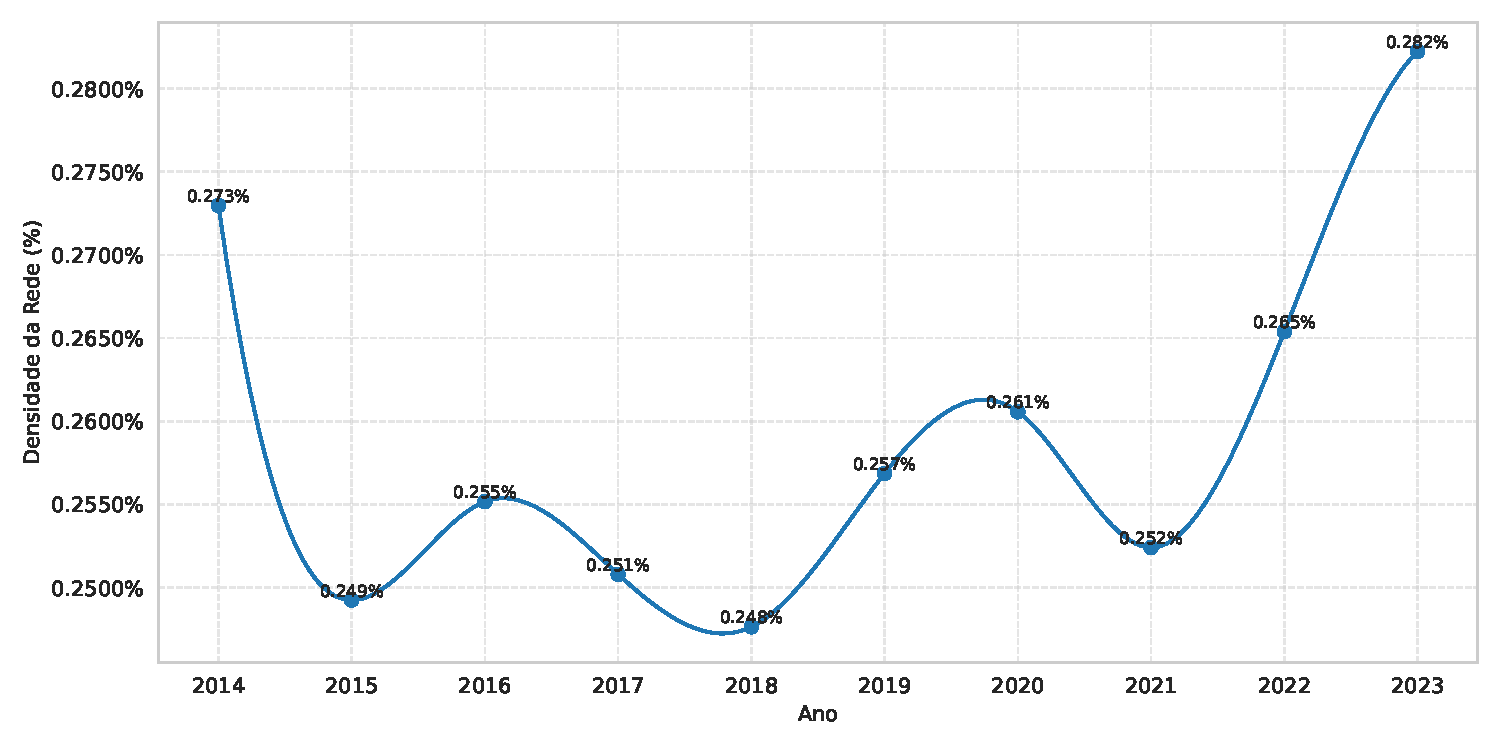
\includegraphics[width=0.9\linewidth]{figuras/density_network.pdf}
    \caption{Densidade rede 2014 a 2023}
    \label{fig:densidade}
\end{figure}

Tabel \ref{tab:densidade} apresenta kona ba porsentu densidade kada tinan husi 2014 a 2023.

\begin{table}[!ht]
    \centering
    \begin{tabular}{|c|c|}
    \hline
        \textbf{Densidade }& \textbf{Tinan } \\ \hline
        0,25\% & 2014 \\ \hline
        0,25\% & 2015 \\ \hline
        %0,21\% & 2016 \\ \hline
        %0,25\% & 2017 \\ \hline
        %0,24\% & 2018 \\ \hline
        %0,26\% & 2023 \\ \hline
    \end{tabular}
    \caption{Densidade por ano}
    \label{tab:densidade}
\end{table}


\section{Análise de rede por programas}
\section{Análise de rede por institucional}
\section{Análise de rede por ano}